%
\documentclass[12pt]{article}
\usepackage[english]{babel}
\usepackage{cite}
\usepackage{amsmath}
%\usepackage[latin1]{inputenc}
%\usepackage[dvips]{graphics}
%\usepackage{graphicx}
%\usepackage{epsfig}
%\usepackage{latexsym}
\usepackage{amssymb}
%\usepackage[T1]{fontenc}
\usepackage{theorem}
\usepackage{algorithmicx}
\usepackage[ruled]{algorithm}
\usepackage{algpseudocode}

\usepackage{graphicx} % figuras
\usepackage{subfigure} % subfiguras


\usepackage[active]{srcltx}
%\numberwithin{equation}{section}
\renewcommand{\theequation}{\arabic{equation}}
\DeclareMathOperator{\e}{e} %La exponencial
\DeclareMathOperator{\sinhc}{sinhc}

\newcommand{\re}[1]{\textrm{#1}} %letra redondilla en f�rmulas matem�ticas
\newcommand{\norm}[1]{\left\Vert#1\right\Vert}
\newcommand{\RE}{\operatorname{Re}}
\newcommand{\IM}{\operatorname{Im}}


\newtheorem{Theorem}{\bf Theorem}[section]
\newtheorem{lemma}{\bf Lemma}%[section]
\newtheorem{definition}{\bf Definition}%[section]
\newtheorem{Corollary}{\bf Corollary}%[section]
\newtheorem{example}{\bf Example}%[section]
\newtheorem{remark}{\bf Remark}%[section]
\newtheorem{proposition}{\bf Proposition}%[section]
\newtheorem{observation}{\bf Note}%[section]
\newtheorem{note}{\bf Note}%[section]

\newenvironment{proof}{\textbf{Proof. \hspace{0.15cm}}}{\hspace*{\fill}$\blacksquare$ \\}




\title{New matrix series expansions for the matrix cosine approximation\footnote{\textbf{Acknowledgements}: This work has been partially supported by Spanish Ministerio
de Econom\'{\i}a y Competitividad and European Regional Development Fund (ERDF) grants
TIN2017-89314-P and by the Programa de Apoyo a la Investigaci\'on y Desarrollo 2018 of the
Universitat Polit\`{e}cnica de Val\`{e}ncia (PAID-06-18) grants SP20180016.
}}
\date{}
\author{Emilio Defez$^{\star}$, Javier Ib\'{a}\~nez$^{\dagger}$, Jos\'e M. Alonso$^{\dagger}$, Pedro Alonso-Jord\'a$^{\natural}$\\
\ \\
\footnotesize  $\star$ Instituto de Matem\'{a}tica Multidisciplinar.\\
\footnotesize  $\dagger$ Instituto de Instrumentaci\'on para Imagen Molecular.\\
\footnotesize  $\natural$ Grupo Interdisciplinar de Computaci\'on y Comunicaciones.\\
\small{Universitat Polit\`{e}cnica de Val\`{e}ncia,} \small{Camino de Vera s/n, 46022, Valencia, Espa\~{n}a.}\\
 \footnotesize  edefez@imm.upv.es, $\left\{\right.$jjibanez, jmalonso,   palonso,$\left.\right\}$@dsic.upv.es}


\begin{document}

\maketitle
\setcounter{page}{1}
\pagestyle{myheadings}
\markboth{Modelling for Engineering \& Human Behaviour 2019\hrulefill}{Modelling for Engineering \& Human Behaviour 2019\hrulefill}
\date{}

\section{Introduction and notation}
In recent years, the study of matrix functions has been the subject of increasing focus due to its usefulness in various areas of
science and engineering, providing new and interesting problems to those already existing and already well-known. Of all matrix functions,
it is certainly the exponential matrix which attracts much of the attention because of its connection with linear first
order differential systems

$$
\left.
\begin{array}{rcl}
Y'(t)&=& AY(t) \\
Y(0)&=& Y_{0} \\
\end{array}\right\} \ , \ A \in \mathbb{C}^{r \times r}
$$
whose solution is given by $Y(t)=e^{A t} Y_{0}$. The hyperbolic matrix functions are applied in the study of the communicability analysis in complex
networks \cite{estrada2008communicability,estrada2005spectral,estrada2016network} and also in the solution of coupled hyperbolic systems
of partial differential equations \cite{jodar2003constructive}. In particular, the trigonometric matrix functions sine and cosine prove especially useful
 in solving systems of second-order linear differential equations of the form:
$$
\left.
\begin{array}{rcl}
\displaystyle \frac{d^2}{dt^2}Y(t)+A^2 Y(t)&=&0 \\
Y(0)&=& Y_{0} \\
Y'(0)&=& Y'_{0} \\
\end{array}\right\} \ , \ A \in \mathbb{C}^{r \times r}
$$
whose solution, if matrix $A$ is non-singular, is given by
$$
Y(t)=\cos{(At)} Y_0+ A^{-1}\sin{(At)}Y'_0.
$$
Due to the relationship $\displaystyle \sin{(A)}=\cos{\left(A + \frac{\pi}{2} I \right)}$, where $I$ is the identity matrix of $\mathbb{C}^{r \times r}$, the
matrix sine can be calculated using the same methods as for the matrix cosine. Usually, research concentrated on approximate calculations of the matrix cosine, 
developing several efficient state-of-the-art algorithms to approximate it. These
methods and algorithms can be found in references \cite{Serb80, dehghan2010computing, High08, alonso2018computing}. Other algorithms, for normal and
nonnegative matrices, based on approximations $L_{\infty}$ also have been presented in Ref. \cite{tsitouras2014bounds}. \\

Among the methods proposed to approximate the matrix cosine, two stand out fundamentally: those based on polynomial approximations (in general based on the
developments of the matrix cosine in Taylor or Hermite series, see \cite{sastre2017two, sastre2019fast, defez2019efficient}) or those based on rational
approximations (i.e. Pad\'e approximation, see \cite{tsitouras2014bounds, Serb79, Serb80, AlHR15}). Normally, polynomial methods are more efficient
in terms of accuracy (although somewhat more computationally expensive) than rational ones.\\

On the other hand, Bernoulli polynomials (and numbers) introduced by Jacob Bernoulli  (1654--1705) in the 18th century, are widely used in various areas of mathematics, both pure and applied, see for example \cite{kouba2013lecture} and references therein.\\

In this paper, we will define Bernoulli matrix polynomials and present a new series expansion of the matrix sine and cosine functions in terms
of these matrix polynomials. Then, we will check that this series expansion will provide a new efficient method to approximate the
matrix cosine.\\

The organization of the paper is as follows: In section \ref{section2}, we will obtain two serial expansions of the matrix cosine in terms of the Bernoulli
matrix polynomials. In section \ref{section4}, we will perform different numerical tests. Conclusions are given in section XXX.\\

Throughout this paper, a polynomial of degree $m$ is given by an expression of the form $P_m(x)=a_{m} x^m+a_{m-1}x^{m-1}+\cdots+a_{1}x+a_{0}$, where $x$ is
the variable (real or complex) and the coefficients $a_j, 0\leq j \leq m$, are complex numbers. Moreover, we can define the matrix polynomial $P_m(B)$ for
$B \in \mathbb{C}^{r \times r}$  as the expression $P_m(B)=a_{m} B^m+a_{m-1}B^{m-1}+\cdots+a_{1}B+a_{0}I$.  As usual, the matrix norm $\left\|\cdots \right\|$
denotes any subordinate matrix norm; in particular $\left\| \cdots \right\|_{1}$ is the usual $1$-norm.

\section{On Bernoulli matrix polynomials}\label{section2}
The sequence of Bernoulli polynomials (denoted by $\left\{B_n(x)\right\}_{n \geq 0}$) and the Bernoulli numbers, $B_n=B_{n}(0)$, appear in important applications for different areas of mathematics, from number theory to classical analysis. For example, they are used for
representing the remainder term of the composite Euler-MacLaurin quadrature rule. They also appear in the Taylor expansion in the neighborhood of the origin of circular and
hyperbolic tangent and co-tangent functions. Moreover, this sequence expresses the exact value of $\zeta(2p)$, with $p$ a positive integer, where $\zeta(z)=\displaystyle \sum_{k \geq 1} \frac{1}{k^{z}}$ is the
well-known Riemann's zeta function. They were first studied by Jacob Bernoulli before 1705 in relation with the computation of sums of
powers of $m$ consecutive integers $\displaystyle S_r(m)=\sum_{k=1}^{m} k^r$, where $r$ and $m$ are two given positive integers. The usual way to define these Bernoulli
polynomials, see \cite[p.~588]{olver2010nist} , is as the coefficients of the Taylor expansion of the following generating function
\begin{equation}\label{Bernoulli1}
g(x, t)= \frac{t e^{tx}}{e^t-1}=\sum_{n \geq 0} \frac{B_n(x)}{n!}t^n  \ , \ |t|<2\pi,
\end{equation}
where $g(x, t)$ is a holomorphic function in $\mathbb{C}$ for the variable $t$ (function $g(x, t)$ has an avoidable singularity in $t=0$). Polynomials $B_n(x)$ have the explicit expression
\begin{equation}\label{Bernoulli2}
B_n(x)=\sum_{k=0}^{n} {n \choose k} B_k x^{n-k},
\end{equation}
where the Bernoulli numbers $B_n$ are defined by the recurrence relation
\begin{equation}\label{Bernoulli3}
B_0=1, \displaystyle  B_{k}= -\sum_{i=0}^{k-1} {k \choose i} \frac{B_i}{k+1-i}, k \geq 1.
\end{equation}
Note that all Bernoulli numbers with impair index vanish, except for $B_{1}=-1/2$. For a matrix $A \in \mathbb{C}^{r \times r}$, we define the $m$-th Bernoulli matrix polynomial by the expression
\begin{equation}\label{Bernoulli4}
B_m(A)=\sum_{k=0}^{m} {m \choose k} B_k A^{m-k}.
\end{equation}
The series expansion of the exponential matrix function $e^{At}$ given by
\begin{equation}\label{Bernoulli5}
e^{At} = \left(\frac{e^t-1}{t}\right)\sum_{n \geq 0} \frac{ B_n(A) t^{n}}{n!} \ , \ 0<|t|<2\pi,
\end{equation}
was demonstrated in Ref. \cite{defez2019}. An efficient method based on formula (\ref{Bernoulli5}) for approximating the exponential matrix has been presented and developed in Ref. \cite{defez2019}.\\

Taking $t=1$ in (\ref{Bernoulli5}) and from the definition of the matrix sine and cosine, it is easy to derive the following expressions
\begin{equation}\label{Bernoulli6}
\left.\begin{array}{rcl}
\cos{(A)} &=&\displaystyle  \left( \cos{(1)}-1\right)\sum_{n \geq 0} \frac{(-1)^n B_{2n+1}(A)}{(2n+1)!}+ \sin{(1)}\sum_{n \geq 0} \frac{(-1)^n B_{2n}(A)}{(2n)!}, \\
\\
\sin{(A)} &=& \displaystyle   \sin{(1)}\sum_{n \geq 0} \frac{ (-1)^n B_{2n+1}(A)}{(2n+1)!}-\left(\cos{(1)}-1\right)\sum_{n \geq 0} \frac{ (-1)^n B_{2n}(A)}{(2n)!}.
\end{array} \right\}
\end{equation}
Replacing in (\ref{Bernoulli5}) the value $t$ for $it$ and $-it$ respectively and taking the arithmetic mean, we can also obtain the result
\begin{equation}\label{Bernoulli7}
\sum_{n \geq 0} \frac{(-1)^n B_{2n}(A)}{(2n)!}t^{2n} =\frac{t}{2 \sin{\left( \frac{t}{2} \right)}}\left(\cos{\left(t A- \frac{t}{2}I \right)}  \right)  \ , \ 0<|t|<2\pi.
\end{equation}
Taking $t=2$ in (\ref{Bernoulli7}), it follows that
\begin{equation}\label{Bernoulli8}
\cos{(A)} = \sin{(1)}\sum_{n \geq 0} \frac{(-1)^n 2^{2n} B_{2n}\left(\frac{A+I}{2}\right)}{(2n)!},
\end{equation}
Note that in formula (\ref{Bernoulli8}) only Bernoulli's polynomials with even index appear, similar to what happens when considering cosine
series expansions using Taylor or Hermite polynomials \cite{sastre2017two,defez2019efficient}.

\section{Algorithms} \label{section3}
If we truncate Expressions \eqref{Bernoulli6} or \eqref{Bernoulli8} of cosine function, then we obtain the following approximation:
\begin{equation}
\label{Pm}
{P_m}(A) = \sum\limits_{i = 0}^m {{p_i^{(m)}}{A^i}},
\end{equation}where the coefficients ${p_i^{(m)}}$ depend on  
 the integer $m$.  These coefficients  converge to the coefficients of the Taylor series when $m$ tends to $\infty$. In Section \ref{section4} three approximations have been considered: two approximations based on Expression  \eqref{Bernoulli6}, an approximation in which all the coefficients are considered and another in which only the coefficients of the even order terms have been considered, and one approximation based on Expression \eqref{Bernoulli8}, where all the coefficients are considered. According to the approaches considered,  two algorithms  has been developed.

\begin{algorithm}[!ht]
\caption{Given a matrix $A \in {\mathbb{C}^{n \times n}}$, this algorithm computes $C=\cos(A)$ by Bernouilli series \eqref{Bernoulli6} or \eqref{Bernoulli8}, where all coefficients have been considered.}
\label{Alg_cos1}
\begin{algorithmic} [1]
\State Select adequate values of $m_k$ and $s \in \mathbb{N} \cup \left\{ 0 \right\}$ \Comment Phase I
\State $A=2^{-s}A$
\State $C=P_{m_k}(A)$ \Comment Phase II: Compute Bernouilli approximation \eqref{Bernoulli6} or \eqref{Bernoulli8} 
 \For {$i=1:s$} \Comment Phase III: Recovering $\cos(A)$
    \State $C=2C^{2}-I$
 \EndFor
\end{algorithmic}
\end{algorithm}

\begin{algorithm}[!ht]
\caption{Given a matrix $A \in {\mathbb{C}^{n \times n}}$, this algorithm computes $C=\cos(A)$ by Bernouilli series \eqref{Bernoulli6}, where only the coefficients of the even order terms have been considered.}
\label{Alg_cos2}
\begin{algorithmic} [1]
\State Select adequate values of $m_k$ and $s \in \mathbb{N} \cup \left\{ 0 \right\}$ \Comment Phase I
\State $A=4^{-s}A^2$
\State $C=P_{m_k}(A)$ \Comment Phase II: Compute Bernouilli approximation \eqref{Bernoulli6}
 \For {$i=1:s$} \Comment Phase III: Recovering $\cos(A)$
    \State $C=2C^{2}-I$
 \EndFor
\end{algorithmic}
\end{algorithm}

In Phase I the integers $m$ and $s$ are
computed so that the Bernouilli approximation of the scaled matrix is computed accurately and efficiently. 
There are several methods can be applied to compute efficiently $C=P_{m_k}(A)$ in Phase II, see ~\cite{PaSt73} and \cite{sastre2018efficient}. In our implementations we used the first one based on  the Paterson-Stockmeyer's
method.
In this method, the integer $m_k$ is chosen from the set
\begin{displaymath}
\label{m_k} \mathbb{M}=\left\{2,4, 6, 9,12,16,20,25,30,36,42,\dots\right\},
\end{displaymath}
where  only the  powers $A^i$, $2\leq i\leq
q$, are computed, being $q = \left\lceil {\sqrt
{{m_k}} } \right\rceil $ or $q=\lfloor \sqrt{m_{k}}\rfloor$ an
integer divisor of $m_{k}$. Then, $C=P_{m_k}(A)$ can
be computed efficiently as
{\setlength\arraycolsep{2pt}{%\small
\begin{align}
\label{PS}
P_{m_k}(A) & =  \\ \nonumber ((( p_{m_k}A^q & +  p_{m_k-1}A^{q-1}
+ p_{m_k-2}A^{q-2}   + \dots + p_{m_k-q+1}A  + p_{m_k-q} I ) A^q \\
\nonumber
               & +  p_{m_k-q-1}A^{q-1} + p_{m_k-q-2}A^{q-2} + \dots + p_{m_k-2q+1}A + p_{m_k-2q} I ) A^q \\ \nonumber
               & +  p_{m_k-2q-1}A^{q-1} + p_{m_k-2q-2}A^{q-2} + \dots + p_{m_k-3q+1}A + p_{m_k-3q} I ) A^q \\ \nonumber
               & \dots  \\ \nonumber
               & +  p_{q-1}A^{q-1} + p_{q-2}A^{q-2} + \dots + p_{1}A + p_{0} I.
\end{align}}}
The computational cost in terms of matrix products of~\eqref{PS} is $\Pi {m_k} = k$.

The computation of the scaling factor $s$ and the order of Bernouilli approximation $m_{k}$  are based on the errors made truncating a series. One first idea is to exploit the sequence $\left\{ {{{\left\| {{A^k}} \right\|}^{1/k}}} \right\}$.
As $\rho (A) \leqslant {\left\| {{A^k}} \right\|^{1/k}} \leqslant \left\| A \right\|$, with $k \geqslant 0$, where $\rho$ is the spectral radius of the matrix $A$, then 
\[\mathop {\lim }\limits_{k \to \infty } ||{A^k}|{|^{1/k}} = \rho (A).\]

Theorem 1.1 from \cite{High09}
shows that if ${h_l} = \sum\limits_{k\geqslant l}^{} {{c_k}{x^k}}$ is a power series with a radius convergence $w$ and ${{\tilde h}_l} = \sum\limits_{k\geqslant l}^{} {\left| {{c_k}} \right|{x^k}}$ , then for any $A \in {\mathbb{C}^{n \times n}}$ 
$$\left\| {{h_l}(A)} \right\| \leqslant {{\tilde h}_l}(||{A^t}|{|^{1/t}}),$$
where $||{A^t}|{|^{1/t}} = \max \left\{ {||{A^k}|{|^{1/k}}:\,\,k \geqslant l,\,\,\,{c_l} \ne 0} \right\}$.

Using the same notation, Theorem 1.1 from \cite{sastre2013exp} shows that if $p_0$ is the multiple of $t$ such that $$l \leqslant {t_0} \leqslant l + p - 1,$$
if $a_{k}$ is an upper bound for $||A^{k}||$ $(||A^{k}||\leq
a_{k})$, $p \in \mathbb{N}$, $1\leq p \leq l$, $p_0\in \mathbb{N}$
is the multiple of $p$ with $l\leq p_0\leq l+p-1$, and
\begin{equation}\label{alphap}
\alpha_{p}=\max\{a_{k}^{\frac{1}{k}}:k=p,l,l+1,l+2,\ldots,p_0-1,p_0+1,p_0+2,\ldots,l+p-1\},
\end{equation}then
%\begin{equation}\label{hlbound}
$||h_{l}(A)||\leq \tilde{h}_{l}(\alpha_{p}).$
%\end{equation}\]

If we apply Theorem 1.1 from \cite{sastre2013exp} for $a_k=||A^{k}||$ and we consider $p=l$, then
$$||h_{l}(A)||\leq \tilde{h}_{l}(\alpha_{l}),$$
where $\alpha_{l}=\max\{||A^{k}||^{\frac{1}{k}}:k=l,l+1,l+2,\ldots,2l-1\}$. This result reduces the values of $||A^{k}||^{\frac{1}{k}}$  given in Theorem 1.1 from \cite{High09}.
In this paper, we propose use the following approximation:
\begin{equation}
\label{Estimation}
\alpha _m \approx ||A^{m}||^{1/m}.
\end{equation}
Using these results, the calculations of $m$ and $s$ from PHASE I of Algorithms \ref{Alg_cos1} and \ref{Alg_cos2} are based on the   relative backward  of
approximating $\cos(A)$ by the approximation \eqref{Pm}.  This error is defined as the matrix $\Delta A$ such that $\cos(A+\Delta A)=P_{m}(A)$. Below, we bound the relative backward error as follows:    
\begin{displaymath}\label{Eb}
E_b=\frac{{\left\| {\Delta A} \right\|}}{{\left\| A \right\|}} =
\frac{{\left\| {\sum\limits_{i \ge0} {{c^{(m)}_i}{A^{^{i+1}}}} }
\right\|}}{{\left\| A \right\|}} \backsimeq\ \frac{{\left\| {\sum\limits_{i \ge m+1} {{c^{(m)}_i}{A^{^{i+1}}}} }
\right\|}}{{\left\| A \right\|}} \le  \left\| {\sum\limits_{i \ge m}
{{c^{(m)}_i}{A^{i}}} } \right\|.
\end{displaymath}
If we define ${h_{m}}(x) = \sum\limits_{i \geqslant m} {{c^{(m)}_i}{x^{i}}} {\text{ }}$ and ${\tilde h_{m}}(x) = \sum\limits_{i \ge
m} {\left| {{c^{(m)}_i}} \right|{x^{i}}} {\rm{ }}$, then
\begin{equation}
E_b \le \left\| {{h_{m}}(A)} \right\| \le {{\tilde h}_{m}}({{\alpha}
_{m}}).
\end{equation}Let $\Theta_{m}$ be
\begin{equation} {\Theta_{m}} = \max \left\{
{{\theta\geq0}:\,\,\sum\limits_{i \ge m} {\left| {{c^{(m)}_i}}
\right|{\theta}^{i}}  \le u} \right\},
\end{equation}
where $u$ is the unit roundoff in IEEE double precision arithmetic ($u=2^{-53}$). For computing $ {\Theta}_{m}$, the MATLAB
Symbolic Math Toolbox has been used.  

On the other hand, if $\alpha_m<\Theta_m$, then
\begin{equation}
{E_b} \leqslant \left\| {{h_m}(A)} \right\| \leqslant {\tilde h_m}(\alpha _m) \leqslant {\tilde h_m}({\Theta _m}) \leqslant u.
\end{equation}
Hence, if $\alpha_m<\Theta_m$, then $E_b\le u$; if not, we would find a value of $s$ such that $2^{-s}\alpha_m<\Theta_m$ (in this case we   compute $P_{m_k}(2^{-s}A)$ in step 3 of Algorithm \ref{Alg_cos1}) or a value of $s$ such that $4^{-s}\alpha_m<\Theta_m$ (in this case we  compute $P_{m_k}(4^{-s}A)$ in step 3 of Algorithm \ref{Alg_cos2}). 

The norms $||A^{m}||^{1/m}$ can be computed approximately using  matrix powers
previously computed  based on the estimation of norms of matrix powers  block 1-norm estimation algorithm
from~\cite{High88}. Taking  into account
that analysis, Algorithms \ref{ms-1}, \ref{ms-2} and \ref{ms-3}  have been developed.  

Algorithms \ref{ms-1} and \ref{ms-2} initially check whether there is a value $m_i$,  $m_{\min}\le m_{i}\le m_{\max}$,
such that $\alpha_{m_{i}} \leq \Theta_{m_{i}}$, computing the necessary powers of matrix $A$  to obtain $P_{i}(A)$ from \eqref{PS} as $i$ increases. The values  of  $m_{\min}$ and $ m_{\max}$ can be  varied in the developed implementations.
 If there is such value $m_i$, then we choose the lower
order $m=m_i$ such that $\alpha_{m_{i}} \leq \Theta_{m_{i}}$ and  $s=0$.
Otherwise, we choose $m=m_{\max}$ and
\begin{equation*}
s = \max \left\{ {0,\left\lceil f_{s}\log \left(
{\frac{{{\alpha_{m_{\max}}}}}{{\Theta_{_{m_{\max}}})}}} \right)
\right\rceil } \right\},
\end{equation*}%Algoritmo EstNormaConPotencias 
where $fs=1$, if Algorithm \ref{Alg_cos1} is used, or  $fs=0.5,$ if Algorithm \ref{Alg_cos2} is used. In Algorithm \ref{ms-1} the lines 20-29 test if it is possible to decrease the above values $s$ and $m$ (the initial value of $m$ is $m_{\max}$), so that
\[{\tilde h_m}(2^{-s}\alpha _m) \leqslant {\tilde h_m}({\Theta _m}) \leqslant u \]
is fulfilled, when Algorithm \ref{Alg_cos1} is used, or \[{\tilde h_m}(4^{-s}\alpha _m) \leqslant {\tilde h_m}({\Theta _m}) \leqslant u\]
 it is fulfilled, when Algorithm \ref{Alg_cos2}.
In those cases, those new values are considered.

In Algorithm \ref{ms-2} the lines 19-24 test if it is possible to decrease the value $s$ so that
  $$|p_{m_{\max}}|a_{m_{\max}}2^{(1-s)m_{\max}}<u,$$
if Algorithm \ref{Alg_cos1} is used, or
$$|p_{m_{\max}}|a_{m_{\max}}4^{(1-s)m_{\max}}<u,$$
if Algorithm \ref{Alg_cos2} is used, where $p_{m_{\max}}$ is the  coefficient of the term of order $m_{\max}$ of Bernouilli series. 

Unlike algorithms \ref{ms-1} and \ref{ms-2}, Algorithm \ref{ms-3} does not compute the powers of matrix $A$, so the estimate \eqref{Estimation} is obtained only from $A$. Algorithm \ref{ms-3} computes $\alpha_m$ such that
\[\left| {\frac{{\alpha_{m_{i}} - \alpha_{m_{i-1}}}}{{\alpha_{m_{i}}}}} \right| < tol,\]
where $tol$ is a small prefixed value (see Lines 3-11).
Then Algorithm \ref{ms-3} check if  $ m_{i}\le m_{\max}$ such that $\alpha_{_{m_{i}}} \leq \Theta_{m_{i}}$. In this case,  we choose the lower
order $m=m_i$ such that $\alpha_{m_{i}} \leq \Theta_{m_{i}}$ and  $s=0$.
Otherwise, we choose $m=m_{\max}$ and
\begin{equation*}
s = \max \left\{ {0,\left\lceil f_s\log \left(
{\frac{{{\alpha_{m_{\max}}}}}{{\Theta_{m_{\max}}})}} \right)
\right\rceil } \right\}.
\end{equation*} 
Next, in the lines 23-32 of Algorithm \ref{ms-3}  is checked if it is possible to decrease the above values $s$ and $m$ so that
\[{\tilde h_m}(2^{-s}\alpha _m) \leqslant {\tilde h_m}({\Theta _m}) \leqslant u \]
is fulfilled, when Algorithm \ref{Alg_cos1} is used, or \[{\tilde h_m}(4^{-s}\alpha _m) \leqslant {\tilde h_m}({\Theta _m}) \leqslant u\]
 it is fulfilled, when Algorithm \ref{Alg_cos2}.
In those cases, those new values are considered.

  \begin{algorithm}[!ht]
\caption{Given a matrix $A \in {\mathbb{C}^{n \times n}}$, a minimum order $m_{\min}\in\mathbb{M}$ and a maximum order $m_{\max}\in\mathbb{M}$, this algorithm calculates an order $m_i\in\mathbb{M}$, $m_{\min}\le m\le m_{\max}$, a factor $s$ and several powers of $A$ for computing $C$ in PHASE II.}
\label{ms-1}
\begin{algorithmic} [1]
\State $A_1=A$; $i=\min$; $f$=0
\While {$f=0$ and $i\le \max$}
    \State $v=\sqrt {m_{i}}$
    \State $j=\left\lceil v\right\rceil$
    \If {$v>j$}
        \State $A_j=A_{j-1}A$ 
    \EndIf
    \State ${\alpha_{m_{i}}} \approx {\left\| {{A^{m_i}}} \right\|^{1/m_i}}$ from $A_j$  \Comment based on Algorithm 1  from~\cite{High88} 
    \If {$\alpha_{m_{i}}<\Theta_{m_{i}}$  }
        \State $f=1$
    \Else
         \State $i=i+1$
    \EndIf 
\EndWhile
\If {$f=1$}
    \State $s=0$
\Else
    \State $s = \left\lceil {\max \left( {0,{{f_{s}\log }_2}({\alpha_{m_{\max}}}/{\Theta_{m_{\max}}})} \right)} \right\rceil $ or  
    \State $j=i_{\min}$
    \State $f=0$
    \While {$f=0$}
       \State $j=j-1$
       \State $s_1 = \left\lceil {\max \left( {0,{{f_{s}\log }_2}({\alpha_{m_{j}}}/{\Theta_{m_{j}}})} \right)} \right\rceil $
       \If {$s\ge s_1$ and $j\geq i_{\min}$}
            \State $s=s_1$
            \State $i=j$
       \Else 
            \State $f=1$  
       \EndIf 
    \EndWhile   
\EndIf
\State $m=m_i$    
\end{algorithmic}
\end{algorithm}

%Algoritmo EstNormaConPotenciasNuevo 
\begin{algorithm}[!ht]
\caption{Given a matrix $A \in {\mathbb{C}^{n \times n}}$, a minimum order $m_{\min}\in\mathbb{M}$ and a maximum order $m_{\max}\in\mathbb{M}$, this algorithm calculates an order $m\in\mathbb{M}$, $m_{\min}\le m\le m_{\max}$, a scaling factor $s$  and the necessary powers of $A$ for computing $C$ in PHASE II.}
\label{ms-2}
\begin{algorithmic} [1]
\State $A_1=A$; $i=\min$; $f$=0
\While {$f=0$ and $i\le \max$} 
    \State $v=\sqrt {m_{i}}$
    \State $j=\left\lceil v\right\rceil$
    \If {$v>j$}
        \State $A_j=A_{j-1}A$ 
    \EndIf
    \State Compute ${a_{m_{i}}} \approx {\left\| {{A^{m_i}}} \right\|}$ from $A^{j}$  \Comment based on Algorithm 1  from~\cite{High88} 
    \State ${\alpha _{{m_i}}} = \sqrt[{{m_i}}]{{{a_{{m_i}}}}}$
    \If {$\alpha_{mi}<\Theta_{m_{i}}$}
        \State $f=1$ 
    \Else
         \State $i=i+1$
    \EndIf
\EndWhile
\If {$f=1$}
    \State $s=0$
\Else
    \State $i=i_{\max}$
    \State $s = \left\lceil {\max \left( {0,{{f_s\log }_2}({\alpha_{m_{i}}}/{\Theta_{mi}})} \right)} \right\rceil $ 
\If {$|p_{m_{i}}|a_{m_{i}}r^{(-s+1)m_{i}}<u$} \Comment $r=2$ (Algorithm \ref{Alg_cos1})
 \State \Comment  $r=4$ (Algorithm \ref{Alg_cos2}) 
    \State $s=s-1$
    \If {$|p_{m_{i}}|a_{m_{i}}r^{(-s+1)m_{i}}<u$}
       \State $s=s-1$
    \EndIf 
\EndIf
\EndIf
\State $m=m_i$    
\end{algorithmic}
\end{algorithm}

%Algoritmo EstNormaSinPotencias 
\begin{algorithm}[!ht]
\caption{Given a matrix $A \in {\mathbb{C}^{n \times n}}$ and a  small value $tol$, this algorithm calculates  calculates an order $m\in\mathbb{M}$, $m_{\min}\le m\le m_{\max}$, and the scaling factor $s$.}
\label{ms-3}
\begin{algorithmic} [1]
\State $i=\min$; $f=0$; 
\State Compute ${\alpha_0} \approx {\left\| {{A^{m_{i}}}} \right\|^{1/m_{i}}}$ from $A$  \Comment based on Algorithm 1  from~\cite{High88}
\While {$f=0$ and $i< \max$}
    \State $i=i+1$ 
    \State Compute ${\alpha} \approx {\left\| {{A^{m_{i}}}} \right\|^{1/m_{i}}}$ from $A$  \Comment based on Algorithm 1  from~\cite{High88}
    \If {$|\alpha-\alpha_0|>\alpha \cdot tol $}
        \State $\alpha_0=\alpha$ 
    \Else
        \State $f=1$
    \EndIf
\EndWhile
\State  $i=\min$; $f=0$ 
\While {$f=0$ and $i\le \max$} 
    \If {$\alpha<\Theta_{m_{i}}$}
        \State $f=1$
    \Else
        \State $i=i+1$
    \EndIf
\EndWhile
\If {$f=1$}
    \State $s=0$
\Else
    \State $i=i_{\max}$
    \State $s = \left\lceil {\max \left( {0,{{f_{s}\log }_2}({\alpha}/{\Theta_{m_{\max}}})} \right)} \right\rceil $ 
    \State $f=0$
    \State $j=i$
    \While {$f=0$}
       \State $j=j-1$
       \State $s_1 = \left\lceil {\max \left( {0,{{f_{s}\log }_2}({\alpha }/{\Theta_{m_{j}}})} \right)} \right\rceil $
       \If {$ s\ge s_1$ }
            \State $s=s_1$
            \State $i=j$
       \Else 
            \State $f=1$  
       \EndIf 
    \EndWhile   
\EndIf
\State $m=m_i$    
\end{algorithmic}
\end{algorithm}

%this algorithm calculates $m$ and $s$ by Bernouilli series \eqref{Bernoulli6}, %where only the coefficients of the even order terms have been considered.}




\section{Numerical Experiments}\label{section4}
Although theoretically, and according to formulation \eqref{Bernoulli8}, all terms occupying odd positions should be equal to 0, in practice it might not happen with all of them. As an example, table \ref{table_coefficients} shows the coefficients of the Bernoulli polynomial $B_m(A)=a_{m} A^m+a_{m-1}A^{m-1}+\cdots+a_{1}A+a_{0}I$ for formulae \eqref{Bernoulli6} and \eqref{Bernoulli8} when m=25. As it can be seen in the third column of the table, most of the odd terms are not equal to 0, although they are close to it. This raises the dilemma of converting these values directly into zero and taking into account only the even terms or keeping them as they are and considering all of them.  
\begin{table}[!t]\begin{center}
                \caption{Bernoulli polynomial coefficientes for m=25.}
{\footnotesize
               \begin{tabular}{|c||c|c|}\hline Coefficients  & Expression \eqref{Bernoulli6}  & Expression \eqref{Bernoulli8}\\\hline
  $a_0$   &     1.000000000000000e+00   &  9.999999999999776e-01 \\\hline
  $a_1$   &     4.268425513808927e-17   &  2.200931543663476e-25 \\\hline
  $a_2$   &    -5.000000000000000e-01   & -4.999999999998889e-01 \\\hline
  $a_3$   &    -7.103351130950067e-18   &  9.114115486610701e-26 \\\hline
  $a_4$   &     4.166666666666666e-02   &  4.166666666657532e-02 \\\hline
  $a_5$   &     3.340635907377075e-19   &  1.642205248036368e-25 \\\hline
  $a_6$   &    -1.388888888888889e-03   & -1.388888888858840e-03 \\\hline
  $a_7$   &     1.188305192257936e-20   &  2.406735243784263e-26 \\\hline
  $a_8$   &     2.480158730158730e-05   &  2.480158729629132e-05 \\\hline
  $a_9$   &    -1.104189679966496e-20   & -2.741989705063794e-28 \\\hline
  $a_{10}$   &    -2.755731922398609e-07  &  -2.755731916590913e-07 \\\hline
  $a_{11}$   &     4.004071095795792e-21  &  -2.506940767309528e-29 \\\hline
  $a_{12}$   &     2.087675698787421e-09  &   2.087675655363431e-09 \\\hline
  $a_{13}$   &    -1.013606842281333e-21  &  -1.827655933239498e-31 \\\hline
  $a_{14}$   &    -1.147074559786225e-11  &  -1.147074324303990e-11 \\\hline
  $a_{15}$   &     1.905862492984388e-22  &  -3.648057207260014e-33 \\\hline
  $a_{16}$   &     4.779477334567797e-14  &   4.779467650734273e-14 \\\hline
  $a_{17}$   &    -2.768223171137328e-23  &   2.331854748958815e-35 \\\hline
  $a_{18}$   &    -1.561920725009726e-16  &  -1.561889490721346e-16 \\\hline
  $a_{19}$   &     3.205121320979757e-24  &                       0 \\\hline
  $a_{20}$  &     4.110320556779777e-19   &  4.109509217914593e-19 \\\hline
  $a_{21}$  &    -3.051721100969466e-25   &                      0 \\\hline
  $a_{22}$  &    -8.897045307814457e-22   & -8.879692513470797e-22 \\\hline
  $a_{23}$  &     2.530017510290091e-26   &                      0 \\\hline
  $a_{24}$  &     1.613667223591245e-24   &  1.582268801402494e-24 \\\hline
  $a_{25}$  &    -2.511873775100074e-27   &                      0  \\\hline
                \end{tabular}}
                \label{table_coefficients}
        \end{center}
\end{table}
 
Therefore, having in mind the expression \eqref{Bernoulli6}, the two different mentioned above alternatives that derive from the expression \eqref{Bernoulli8} and the three distinct algorithms, described in section \ref{section3}, to compute the polynomial degree $m$ and the scaling parameter $s$, nine different approximations are given in this paper to compute cosine matrix function. To test and compare the numerical performance of all these different approaches, the following algorithms have been implemented on MATLAB R2018b:

\begin{description}
\item $\bullet$ \emph{cosmber\_1\_3}, \emph{cosmber\_1\_4} and \emph{cosmber\_1\_5}: codes based on formula \eqref{Bernoulli6}, where all the polynomial terms must be considered. Algorithms \ref{ms-1}, \ref{ms-2} and \ref{ms-3} will be used in each code, respectively, to compute $m \in \left\{ {30, 36} \right\}$ and $s$ values.  

\item $\bullet$ \emph{cosmber\_2\_3}, \emph{cosmber\_2\_4} and \emph{cosmber\_2\_5}: implementations belonging to formula \eqref{Bernoulli8}. As in the previous case, even and odd terms will be taken into account. Algorithms \ref{ms-1}, \ref{ms-2} and \ref{ms-3} will be also respectively considered to calculate $m \in \left\{ {30, 36} \right\}$ and $s$ parameters.

\item $\bullet$ \emph{cosmber\_3\_3}, \emph{cosmber\_3\_4} and \emph{cosmber\_3\_5}: developments derived from formula \eqref{Bernoulli8} where odd position terms have been neglected. In this way, only the even terms will be employed, as in the case of Taylor series occur \cite{sastre2017two}. One more time, the same algorithms \ref{ms-1}, \ref{ms-2} and \ref{ms-3} will be employed to work out $m \in \left\{ {16, 20} \right\}$ (it would be equivalent to $m=32$ or $40$ using the even and odd terms) and $s$.  

\item $\bullet$ \emph{cosm}: implementation based on the Pad\'e rational approximation for the cosine matrix function\cite{AlHR15}.

\end{description}

MATLAB's Symbolic Math Toolbox with 256 digits of precision was run to compute the exact matrix cosine function, using the vpa (variable-precision floating-point arithmetic) function.

The next test battery, composed of three types of different and representative matrices, have been used to compare the above mentioned algorithms:

\begin{description}
\item[a)] \textbf{Diagonalizable real matrices}: they have been obtained as $A=V \cdot D \cdot V^{-1}$,
where $D$ is a diagonal matrix (with real and complex eigenvalues) and matrix $V$ is an orthogonal matrix, $V=H/\sqrt{n}$, being $H$ a Hadamard matrix and $n$ its number of rows or columns.
We have $2.18 \leq \left\|A \right\|_1 \leq 132.62$. The matrix cosine was exactly calculated as $\cos{(A)}=V \cdot \cos{(D)} \cdot V^{T}$.

\item[b)] \textbf{Non-diagonalizables complex matrices}: they have been computed as $A=V \cdot J \cdot V^{-1}$, where
$J$ is a Jordan matrix with complex eigenvalues with module less than $10$ and random algebraic multiplicity between $1$ and $5$. $V$ is an orthogonal random
matrix with elements in the interval $[-0.5,0.5]$. We have $91.3 \leq \left\|A \right\|_1 \leq 92.6$. The {\it``exact"} matrix cosine was computed as $\cos{(A)}=V \cdot \cos{(J)} \cdot V^{-1}$.

\item[c)] \textbf{Matrices from the Matrix Computation Toolbox (MCT)} \cite{higham1995test} and from the \textbf{Eigtool MATLAB Package (EMP)} \cite{wright2009eigtool}: they have been chosen because they have highly different and significant   characteristics from each other. The {\it``exact"} matrix cosine for these matrices was computed by using Taylor approximations of different orders, changing their scaling parameter.
\end{description}

In the numerical experiments, we used successfully $179$ matrices of size $128\times 128$: $60$ from the diagonalizable set, $60$ from the non-diagonalizable group, $42$ from the MCT and $17$ from the EMP. Although the Matrix Computation Toolbox and the Eigtool Matlab Package are initially composed of fifty-two and twenty matrices, respectively, ten from the MCT and three from the EMP matrices were discarded for different reasons. For example, matrices 5, 15, 16, 17, 21, 42, 43, 44 and 49 belonging to the MCT and matrix 3 from the EMP were not taken into account since the exact cosine solution could not be computed. Besides, matrix 2 from the MCT and matrices 4 and 10 from the EMP were not considered because the excessively high relative error provided by all the methods to be compared.

Initially, three experiments, called Tests, have been independently performed to evaluate the distinct variations of each theoretical formulation, taking into account the corresponding approaches related to algorithms \ref{ms-1}, \ref{ms-2} and \ref{ms-3} to compute $m$ and $s$ parameters. All these executions have been carried out by means of MATLAB (R2018b) running on an HP Pavilion dv8 Notebook PC with an Intel Core i7 CPU Q720 @1.60Ghz processor and 6 GB of RAM.

In the first test, \emph{cosmber\_1\_3}, \emph{cosmber\_2\_3} and \emph{cosmber\_3\_3} codes have been compared to obtain the most appropiate theoretical approach when the algorithm \ref{ms-1} is used. 

Results are given in Tables \ref{tabla_er_comparative_test_todo} and \ref{tabla_er_comparative_test_todoa}. The rows of each table show the percentage of cases in which the relative errors of \texttt{cosmber} (Bernoulli) is lower, greater or equal than the relative errors of \texttt{cosmtay} (Taylor), \texttt{cosmtayher} (Hermite)  and  \texttt{cosm} (Pad\'e). Graphics of the Normwise relative errors and the Performance Profile are given in Figures \ref{fig:todo} and \ref{fig:todoa}. The total number of matrix products was: $3202$ (\emph{cosmber}), $2391$ (\emph{cosmtay}), $1782$ (\emph{cosmtayher}) and  $3016$ (\emph{cosm}). Recall that in the Bernoulli implementation, the maximum value of $m$ to be used was $m=36$ considering all the terms and, in the rest of algorithms, was $m=32$ but just having into account the even terms.


\begin{table}[H]
\hspace{-1cm}
\begin{minipage}[b]{0.55\linewidth} %Una minip�gina que cubre la mitad de la p�gina
\centering
\begin{table}[H]\begin{center}
\caption{Using approximation \eqref{Bernoulli6}}
\resizebox{\textwidth}{!}{
\begin{tabular}{cc}\hline
$E(cosmber)<E(cosmtay)$ & $55.60\%$  \\\hline
$E(cosmber)>E(cosmtay)$ & $44.40\%$ \\\hline
$E(cosmber)=E(cosmtay)$  & $0\%$ \\\hline
$E(cosmber)<E(cosmtayher)$ & $50.97\%$ \\\hline
$E(cosmber)>E(cosmtayher)$ & $49.03\%$ \\\hline
$E(cosmber)=E(cosmtayher)$  & $0\%$ \\\hline
$E(cosmber)<E(cosm)$ & $76.83\%$ \\\hline
$E(cosmber)>E(cosm)$ & $23.17\%$ \\\hline
$E(cosmber)=E(cosm)$  & $0\%$ \\\hline
\end{tabular}
}
\label{tabla_er_comparative_test_todo}
\end{center}
\end{table}
\end{minipage}
\hspace{0.35cm} % Si queremos tener un poco de espacio entre las dos figuras
\begin{minipage}[b]{0.55\linewidth}
\centering
\begin{table}[H]\begin{center}
\caption{Using approximation \eqref{Bernoulli8}}
\resizebox{\textwidth}{!}{
\begin{tabular}{cc}\hline
$E(cosmber)<E(cosmtay)$ & $65.64\%$ \\\hline
$E(cosmber)>E(cosmtay)$ & $34.36\%$ \\\hline
$E(cosmber)=E(cosmtay)$  & $0\%$ \\\hline
$E(cosmber)<E(cosmtayher)$ & $60.62\%$ \\\hline
$E(cosmber)>E(cosmtayher)$ & $39.38\%$ \\\hline
$E(cosmber)=E(cosmtayher)$  & $0\%$ \\\hline
$E(cosmber)<E(cosm)$ & $73.75\%$ \\\hline
$E(cosmber)>E(cosm)$ & $26.25\%$ \\\hline
$E(cosmber)=E(cosm)$  & $0\%$ \\\hline
\end{tabular}
}
\label{tabla_er_comparative_test_todoa}
\end{center}
\end{table}
\end{minipage}
\end{table}
\begin{figure}[htbp]
\centering
\subfigure[Using formula \eqref{Bernoulli6}]{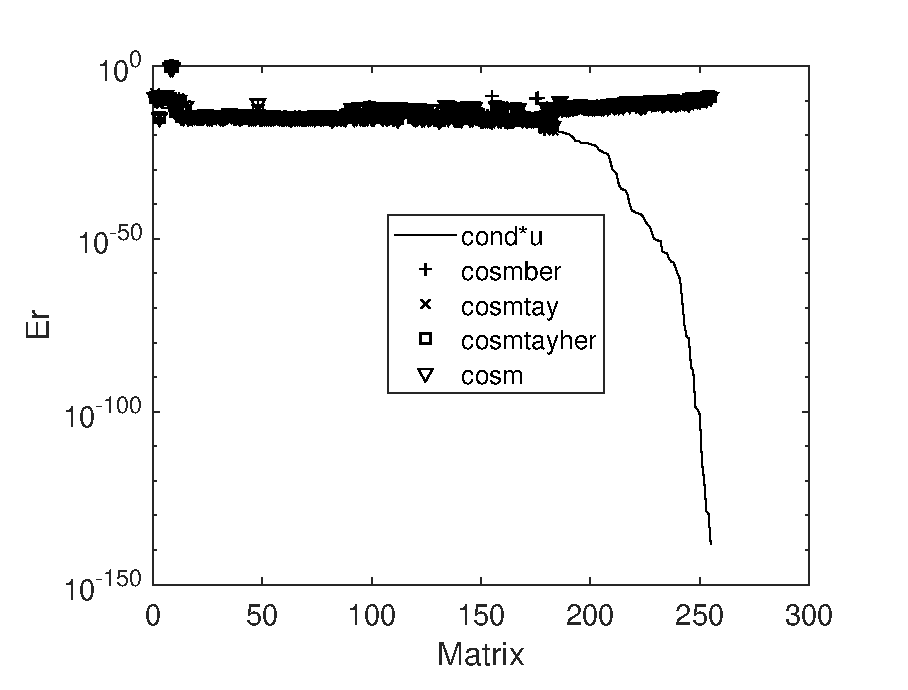
\includegraphics[scale=0.42]{Fig_normwise_9.eps}} %width=40mm
\subfigure[Using formula \eqref{Bernoulli8}]{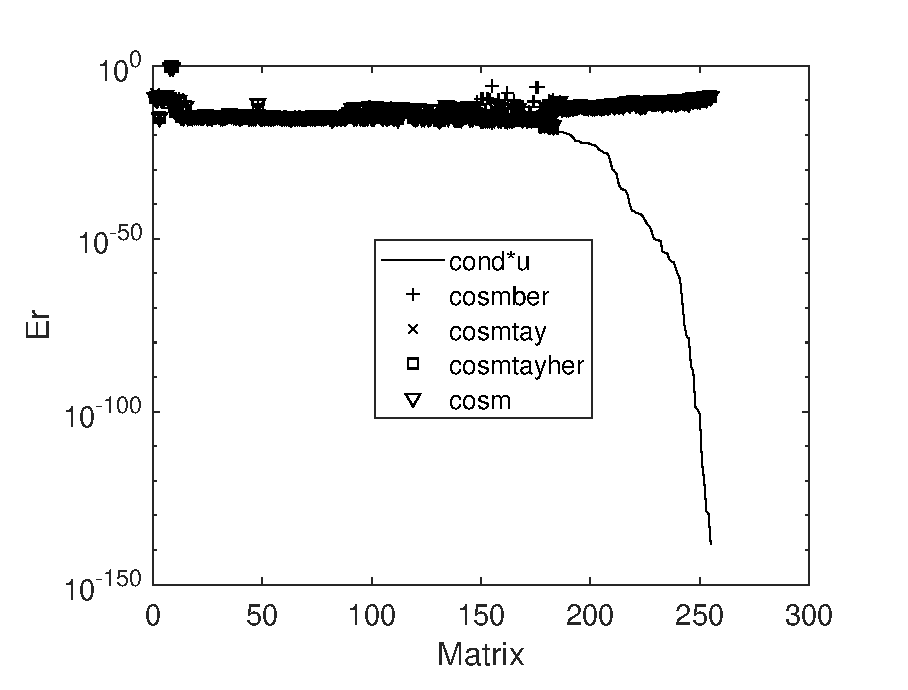
\includegraphics[scale=0.42]{Fig_todas_normwise.eps}}
\caption{Normwise relative errors.} \label{fig:todo}
\end{figure}


\begin{figure}[htbp]
\centering
\subfigure[Using formula \eqref{Bernoulli6}]{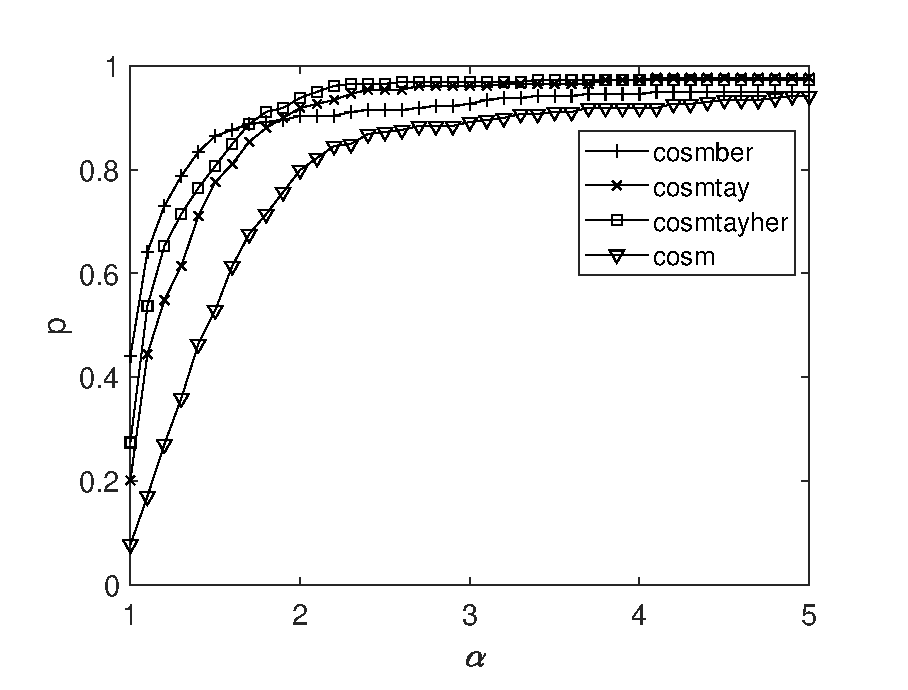
\includegraphics[scale=0.42]{Fig_todas_nprofile_9.eps}} %width=40mm
\subfigure[Using formula \eqref{Bernoulli8}]{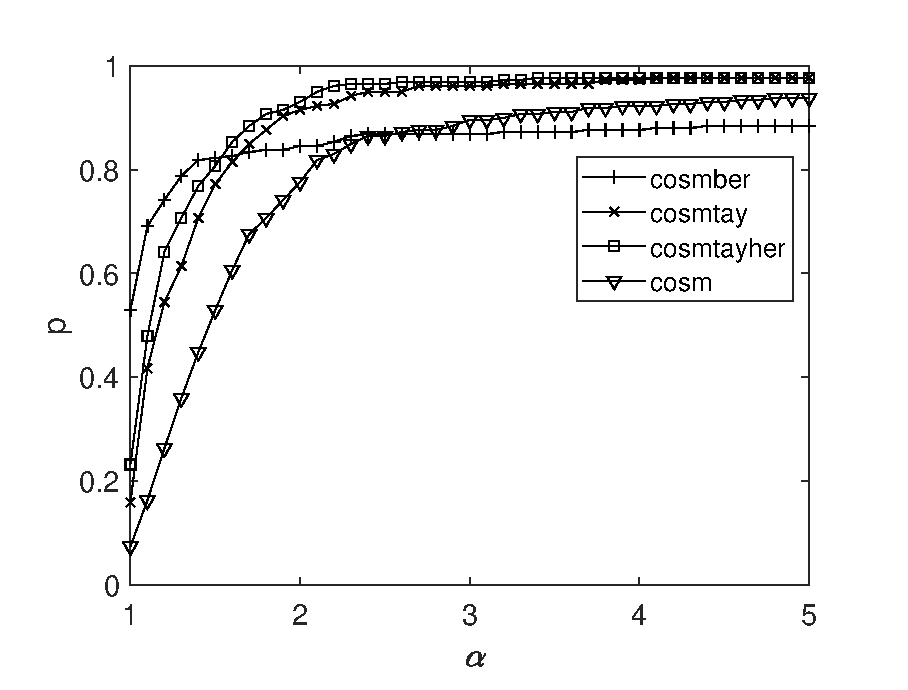
\includegraphics[scale=0.42]{Fig_todas_nprofile.eps}}
\caption{Performance Profile.} \label{fig:todoa}
\end{figure}

\section{Conclusions}\label{section5}
In general, the implementation based on the new Bernoulli series (\ref{Bernoulli6})  is more accurate than (\ref{Bernoulli8}), 
comparing it with the one based on the Taylor series, algorithm  (\texttt{cosmtay}) and Hermite series, algorithm   (\texttt{cosmtayher}), 
and the one based in Pad\'e  rational approximation, algorithm (\texttt{cosm}).

\bibliographystyle{unsrt}
\bibliography{bib_imm2019}
\end{document}
